\documentclass[crop,tikz]{standalone}                 
\usepackage{physics}
\makeatletter                                                                                        

\newcommand{\sq}[1]{\frac{1}{\sqrt{#1}}}

\begin{document}

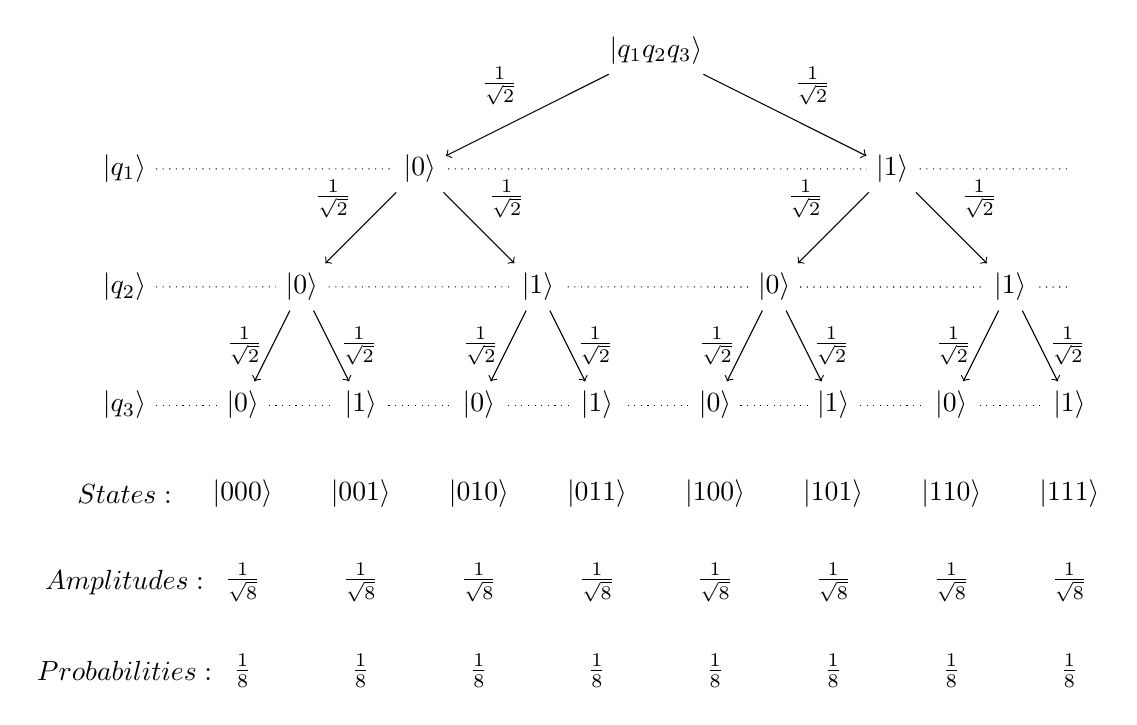
\begin{tikzpicture}[scale=1.5]                                                                          
%\draw [dotted] (0,0) grid (8, 3);

% qubit lines
\node [] (nodeq1) at ( +0.00, +2.00) {$\ket{q_1}$};                                           
\node [] (nodeq2) at ( +0.00, +1.00) {$\ket{q_2}$};                                           
\node [] (nodeq3) at ( +0.00, +0.00) {$\ket{q_3}$};                                           

\draw [dotted] (nodeq1) -- ( +8.00, +2.00);
\draw [dotted] (nodeq2) -- ( +8.00, +1.00);
\draw [dotted] (nodeq3) -- ( +8.00, +0.00);

% states / configurations
\node [] (nodere) at ( +0.00, -0.75) {$States:$}  ;                                           
\node [] (noder1) at ( +1.00, -0.75) {$\ket{000}$};                                           
\node [] (noder2) at ( +2.00, -0.75) {$\ket{001}$};                                           
\node [] (noder3) at ( +3.00, -0.75) {$\ket{010}$};                                           
\node [] (noder4) at ( +4.00, -0.75) {$\ket{011}$};                                           
\node [] (noder5) at ( +5.00, -0.75) {$\ket{100}$};                                           
\node [] (noder6) at ( +6.00, -0.75) {$\ket{101}$};                                           
\node [] (noder7) at ( +7.00, -0.75) {$\ket{110}$};                                           
\node [] (noder8) at ( +8.00, -0.75) {$\ket{111}$};                                           

% amplitudes
\node [] (nodeam) at ( +0.00, -1.50) {$Amplitudes:$} ;                                           
\node [] (nodea1) at ( +1.00, -1.50) {$\sq{8}$}      ;                                           
\node [] (nodea2) at ( +2.00, -1.50) {$\sq{8}$}      ;                                           
\node [] (nodea3) at ( +3.00, -1.50) {$\sq{8}$}      ;                                           
\node [] (nodea4) at ( +4.00, -1.50) {$\sq{8}$}      ;                                           
\node [] (nodea5) at ( +5.00, -1.50) {$\sq{8}$}      ;                                           
\node [] (nodea6) at ( +6.00, -1.50) {$\sq{8}$}      ;                                           
\node [] (nodea7) at ( +7.00, -1.50) {$\sq{8}$}      ;                                           
\node [] (nodea8) at ( +8.00, -1.50) {$\sq{8}$}      ;                                           

% probabilities
\node [] (nodepr) at ( +0.00, -2.25) {$Probabilities:$};                                           
\node [] (nodep1) at ( +1.00, -2.25) {$\frac{1}{8}$}   ;                                           
\node [] (nodep2) at ( +2.00, -2.25) {$\frac{1}{8}$}   ;                                           
\node [] (nodep3) at ( +3.00, -2.25) {$\frac{1}{8}$}   ;                                           
\node [] (nodep4) at ( +4.00, -2.25) {$\frac{1}{8}$}   ;                                           
\node [] (nodep5) at ( +5.00, -2.25) {$\frac{1}{8}$}   ;                                           
\node [] (nodep6) at ( +6.00, -2.25) {$\frac{1}{8}$}   ;                                           
\node [] (nodep7) at ( +7.00, -2.25) {$\frac{1}{8}$}   ;                                           
\node [] (nodep8) at ( +8.00, -2.25) {$\frac{1}{8}$}   ;                                           

% quantum state tree
\node [fill=white] (nodexxx) at ( +4.50, +3.00) {$\ket{q_1q_2q_3}$};                                           
\node [fill=white] (node0xx) at ( +2.50, +2.00) {$\ket{0}$};                                       
\node [fill=white] (node1xx) at ( +6.50, +2.00) {$\ket{1}$};                                       
\node [fill=white] (node00x) at ( +1.50, +1.00) {$\ket{0}$};                                       
\node [fill=white] (node01x) at ( +3.50, +1.00) {$\ket{1}$};                                       
\node [fill=white] (node10x) at ( +5.50, +1.00) {$\ket{0}$};                                       
\node [fill=white] (node11x) at ( +7.50, +1.00) {$\ket{1}$};                                       
\node [fill=white] (node000) at ( +1.00, +0.00) {$\ket{0}$};
\node [fill=white] (node001) at ( +2.00, +0.00) {$\ket{1}$};                                       
\node [fill=white] (node010) at ( +3.00, +0.00) {$\ket{0}$};                                       
\node [fill=white] (node011) at ( +4.00, +0.00) {$\ket{1}$};                                       
\node [fill=white] (node100) at ( +5.00, +0.00) {$\ket{0}$};                                       
\node [fill=white] (node101) at ( +6.00, +0.00) {$\ket{1}$};                                       
\node [fill=white] (node110) at ( +7.00, +0.00) {$\ket{0}$};                                       
\node [fill=white] (node111) at ( +8.00, +0.00) {$\ket{1}$};                                       

\draw [->] (nodexxx) -- (node0xx) node[midway, above left  ] {$\sq{2}$};
\draw [->] (nodexxx) -- (node1xx) node[midway, above right ] {$\sq{2}$};                                                           
\draw [->] (node0xx) -- (node00x) node[midway, above left  ] {$\sq{2}$};                                                           
\draw [->] (node0xx) -- (node01x) node[midway, above right ] {$\sq{2}$};                                                           
\draw [->] (node1xx) -- (node10x) node[midway, above left  ] {$\sq{2}$};                                                           
\draw [->] (node1xx) -- (node11x) node[midway, above right ] {$\sq{2}$};                                                           
\draw [->] (node00x) -- (node000) node[midway, left  ] {$\sq{2}$};                                                           
\draw [->] (node00x) -- (node001) node[midway, right ] {$\sq{2}$};                                                           
\draw [->] (node01x) -- (node010) node[midway, left  ] {$\sq{2}$};                                                           
\draw [->] (node01x) -- (node011) node[midway, right ] {$\sq{2}$};                                                           
\draw [->] (node10x) -- (node100) node[midway, left  ] {$\sq{2}$};                                                           
\draw [->] (node10x) -- (node101) node[midway, right ] {$\sq{2}$};                                                           
\draw [->] (node11x) -- (node110) node[midway, left  ] {$\sq{2}$};                                                           
\draw [->] (node11x) -- (node111) node[midway, right ] {$\sq{2}$};                                  

\end{tikzpicture}                                                                                   i
 

\end{document}
